\section{Appendices}

% Appendices (if any) -- listings, screen shots, diagrams, etc. 

% Final Remarks: 
% Your advisor may ask you to rewrite your reports. While re-writing the 
% reports: 
% Remove text that is not yours! Cut-n-pasted tutorials, web material, etc. is 
% not part of your report!  
% Write in detail, of what you've done in your summer practice. Using a step-
% by-step progress is a good way to do this.  
% Remove pages of source-code. Use screen shot, whose content explained in 
% captions, and other figures that contributed.  
% Properly format your reports!  
% The reports that are not written properly will be graded as unsatisfactory.

\begin{figure*}[b!]
    \centering
    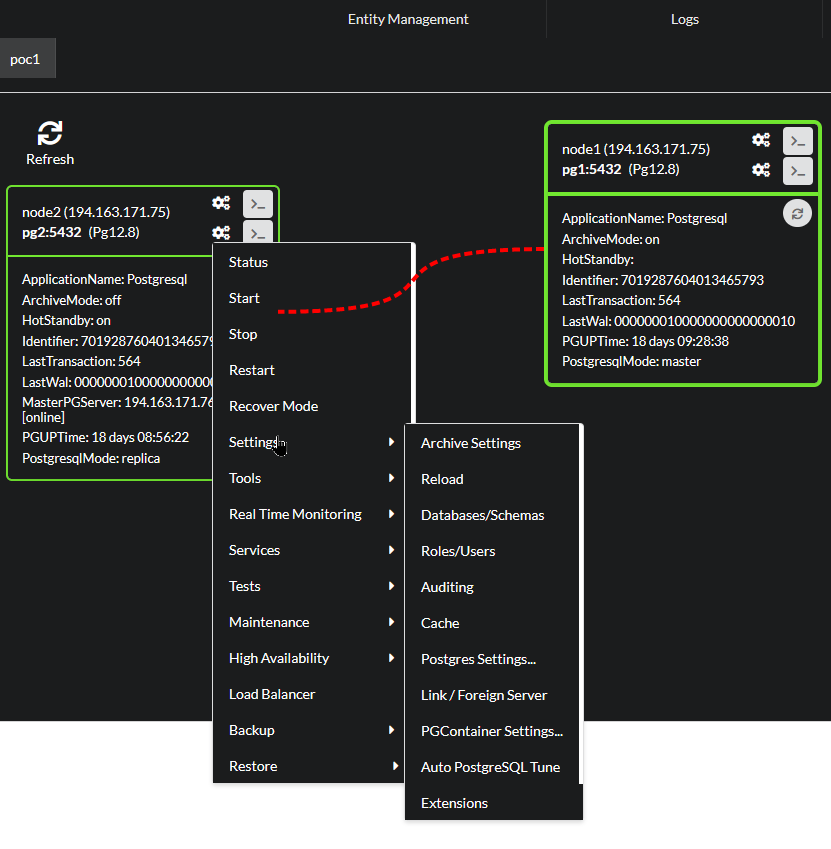
\includegraphics[width=11cm]{classic_container_menu.png}
    \caption{Container view with classic menu.}
\end{figure*}

\begin{figure*}[b!]
    \centering
    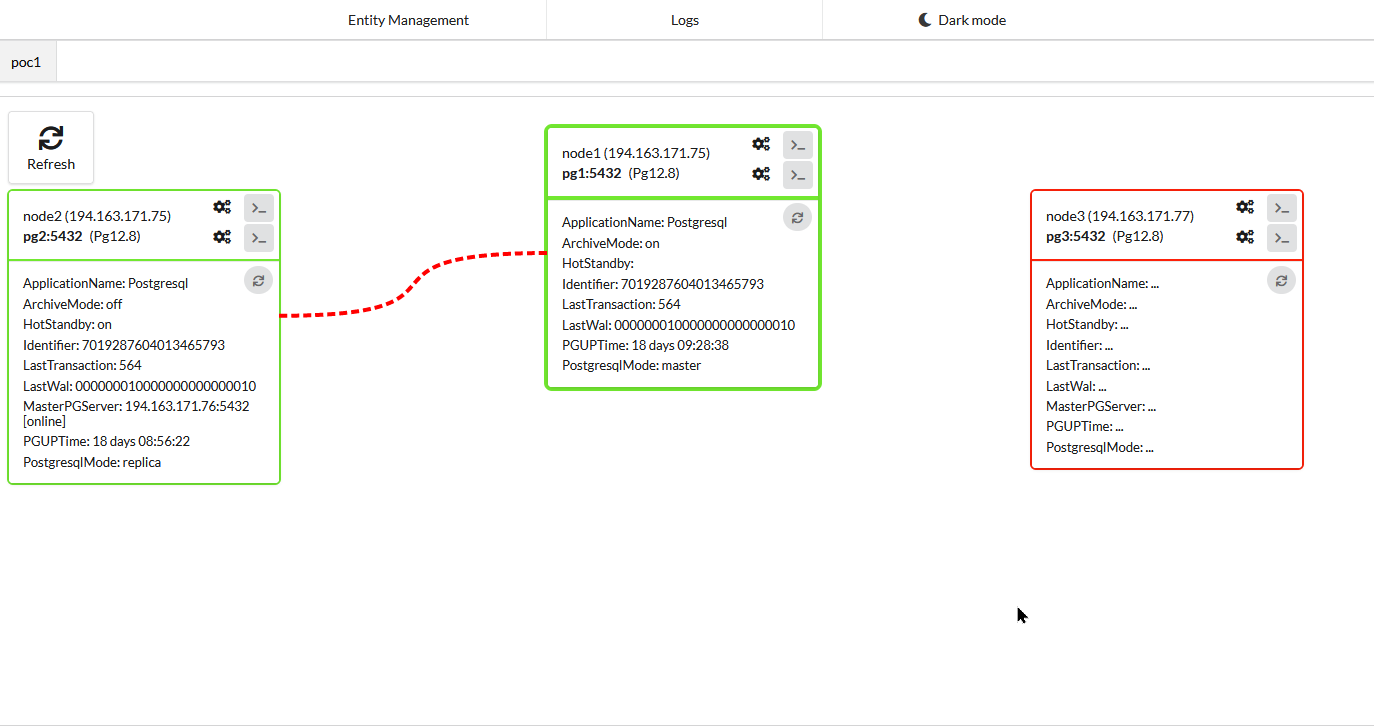
\includegraphics[width=11.5cm]{light_mode_topology.png}
    \caption{Light mode.}
\end{figure*}

\begin{figure*}[b!]
    \centering
    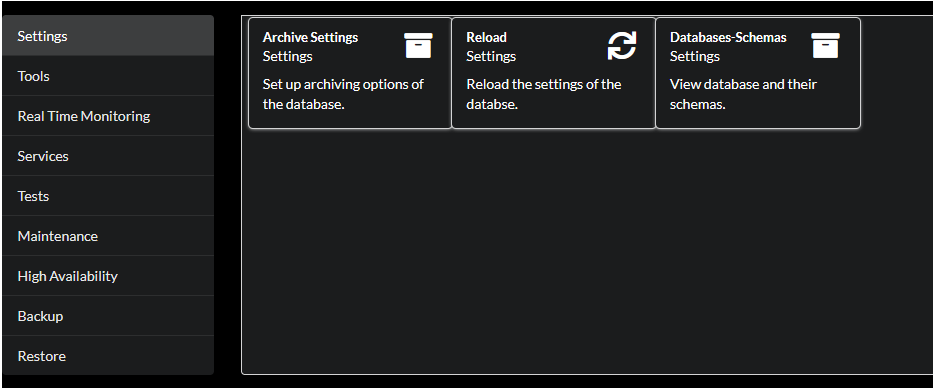
\includegraphics[width=11cm]{alternative_actions_panel.png}
    \caption{An alternative container action menu.}
\end{figure*}

\begin{figure*}[b!]
    \centering
    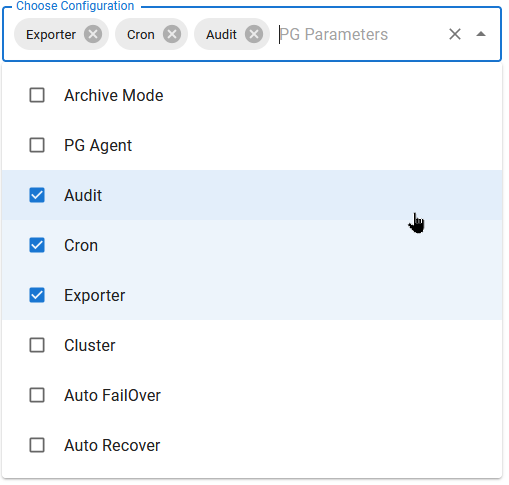
\includegraphics[width=11cm]{container_config_selection.png}
    \caption{Container configuration widget.}
\end{figure*}

\begin{figure*}[b!]
    \centering
    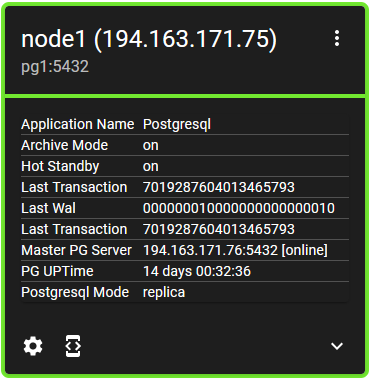
\includegraphics[width=11cm]{mui_container_node.png}
    \caption{Container node view rewritten using Material UI.}
\end{figure*}

\begin{figure*}[b!]
    \centering
    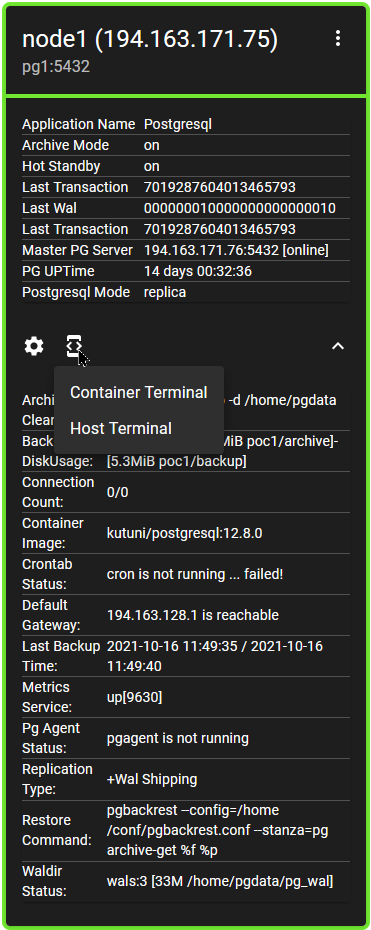
\includegraphics[width=11cm]{mui_container_node_extended.png}
    \caption{MUI container view (extended)}
\end{figure*}

\begin{figure*}[b!]
    \centering
    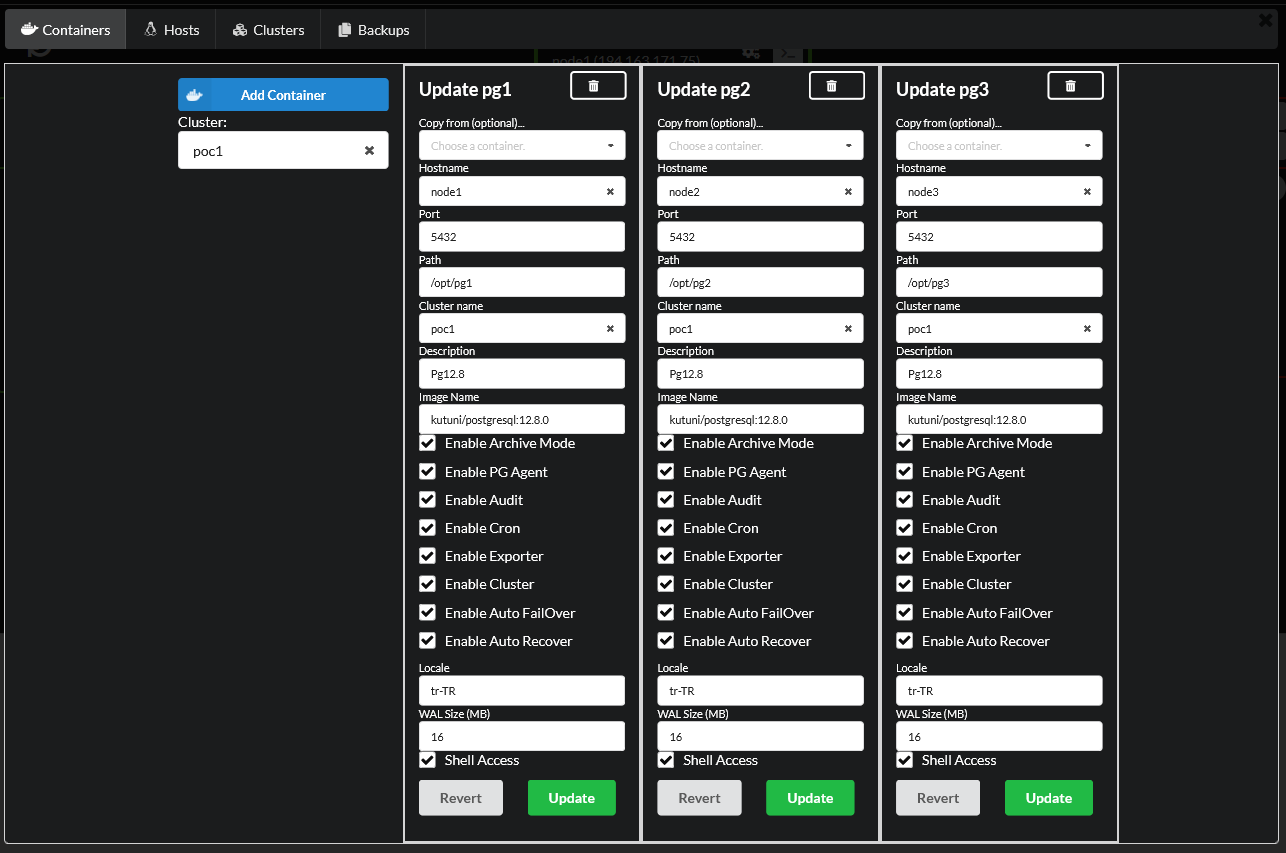
\includegraphics[width=11cm]{entity_management_panel.png}
    \caption{Entity management view.}
\end{figure*}

\begin{figure*}[b!]
    \centering
    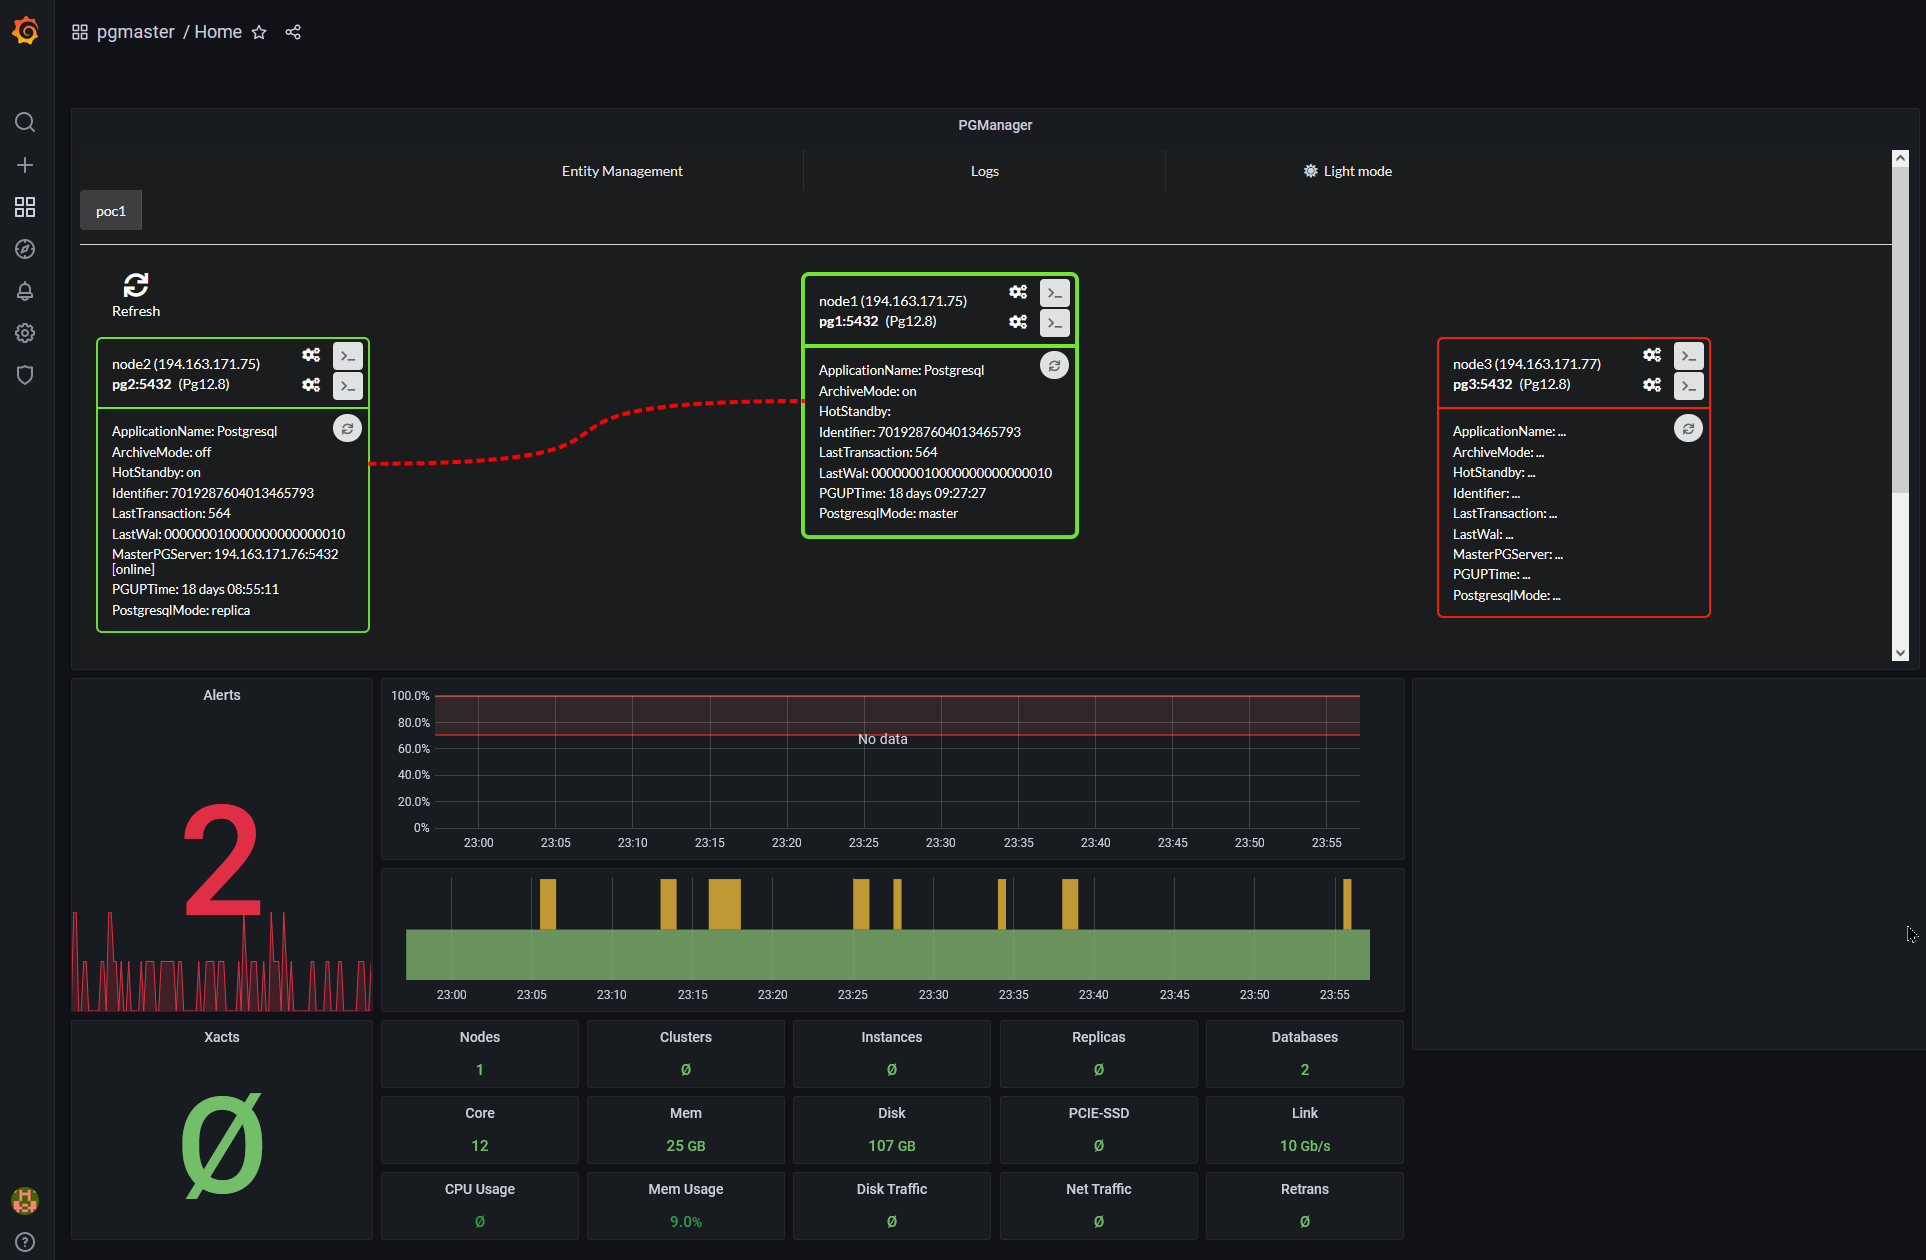
\includegraphics[width=11cm]{pgm_in_grafana.png}
    \caption{PG-Web within Grafana.}
\end{figure*}